\documentclass[tesi]{subfiles}
\IfEq{\jobname}{\detokenize{tesi}}{}{%
    \externaldocument{Chapter1}
}

\begin{document}
	\chapter{International Roughness Index}
\label{ch:IRI}
The International Roughness Index (IRI) \cite{sayers1986guidelines}, was introduced in 1986 by The World Bank(\cite{sayers1986guidelines}, \cite{sayers1986international}). It represents the most used road roughness index to evaluate and manage road infrastructure. 


IRI is defined as the ratio between the sum of vehicle-wheel displacements of a standard vehicle, travelling at \num{80} \si{\km\per\hour} along a roadway\cite{sayers1995calculation}. It is calculated using the \textit{"quarter-car"} mathematical model, whose response is accumulated in order to produce a roughness index\cite{little_book} with slope units ( in  mile$^{-1}$ , $\si{\meter\per\km}$  etc...) 
The measurement of IRI is required for all the data provided to the United States Federal Highway Administration, and it is covered by several standards from ASTM International, such as the ASTM E1364 - 95 (2005)\cite{astm2}. In addition, the IRI is also used to evaluate a new pavement construction, i.e. to determine penalties or bonus payments based on its smoothness.

\section{History}\label{sc:IRI_History}
In the early $1980s$, in the United States of America, some highway engineering companies identified the road roughness as the main indicator to determine the level of comfort of a road network used by different road users, from pedestrians to driver. 
There were already some methodologies used to determine the roughness at that time, however, they were different among the various agencies and neither reproducible or stable over time. 
For this reason, the United States National Cooperative Highway Research Program (NCHRP) started a research project in order to help the state agencies to improve the utilisation of their own methodology for evaluating the road roughness\cite{gillespie1980calibration}. The project was then continued by The World Bank\cite{sayers1986guidelines} under the name of \textbf{\textit{International Road Roughness Experiment}} (IRRE)\cite{sayers1986internationalscale}, whose main goal was to determine a way to compare or to convert the data obtained from different countries, all involved in The World Bank's projects.
After several studies, the results showed that the majority of used methodologies and instruments were able to produce significant measurements\cite{sayers1986international} of road roughness. Thus, all those methodologies were standardised and the measurement was referenced to a single, common scale.
Sayers and Karamihas\cite{little_book} proposed a scale, shown below, where the IRI level is related to the characteristics of a surface and to its degradation. This scale, whose name is International Roughness Index (IRI), was, in fact, first defined and then tested only for this purpose.

\begin{figure}[H]
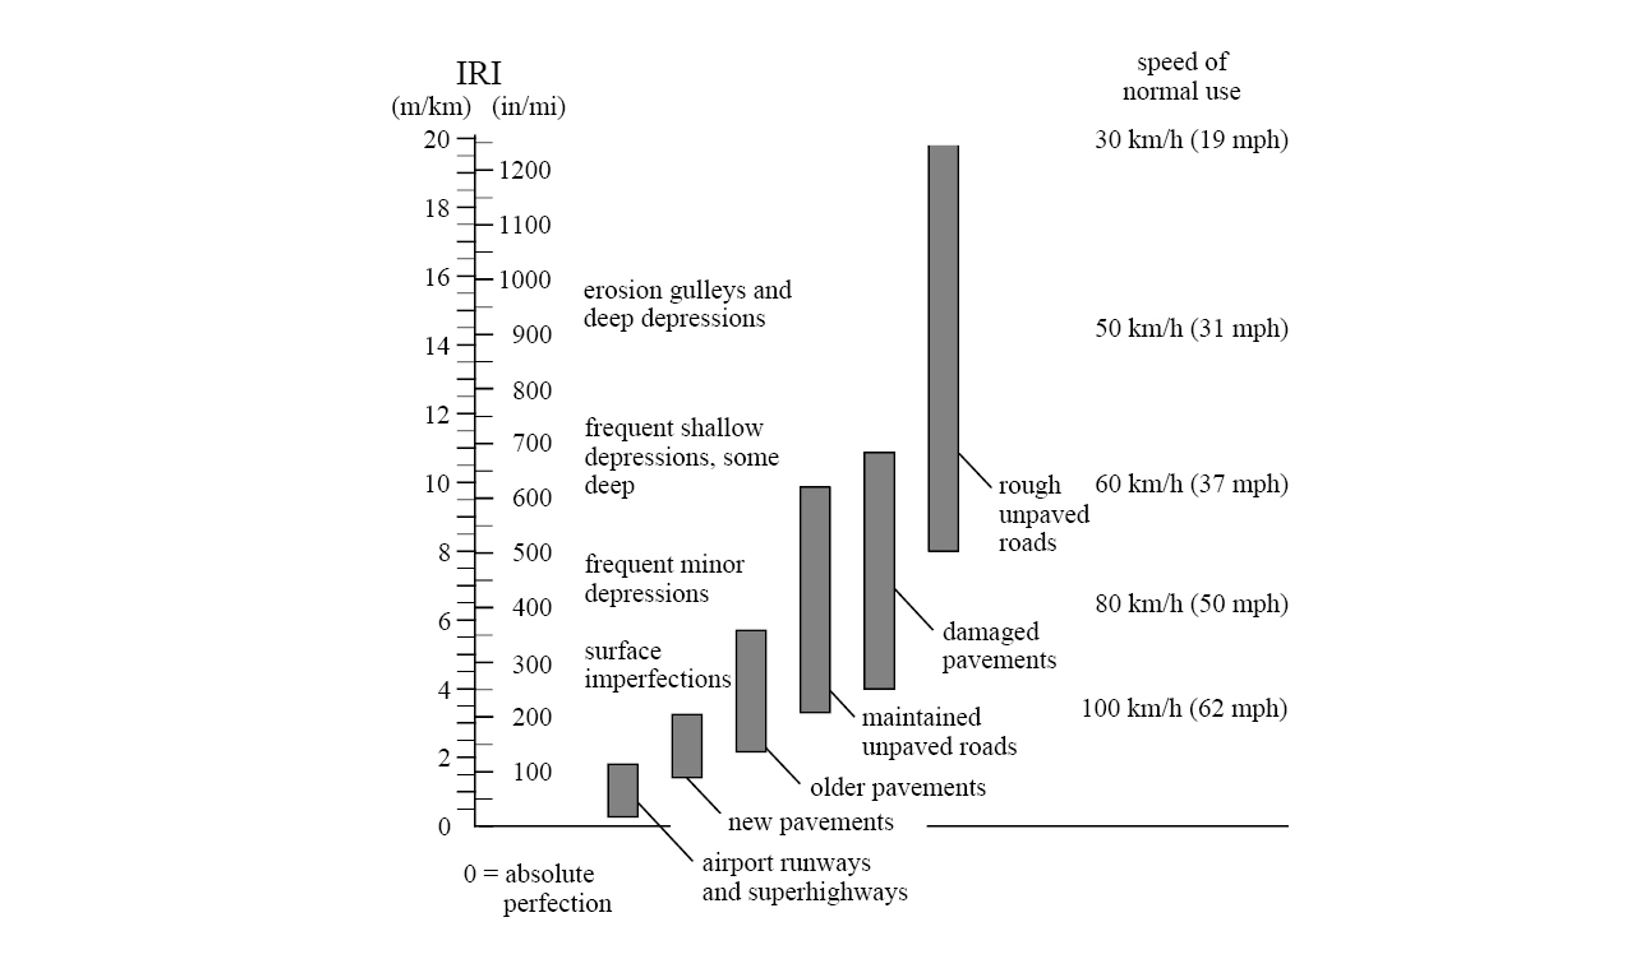
\includegraphics[scale=1]{iri_scale}
\caption{International Roughness Index Scale defined by Sayers and Karamihas \cite{little_book}
Representing the characteristic of road roughness in function of IRI.}
\label{fig:International Roughness Index Scale}
\end{figure}
\clearpage
\section{Definition}\label{sc:IRI Definition}
IRI is defined as a mathematical model of a bidimensional road profile. This road profile represents the vertical elevation of the road surface as a function of the longitudinal distance along the travelling distance\cite{wang2006road}. So, its aim is to show how the elevation varies depending on the length of the road in question.
The roughness measurement is difficult and complex because it depends on the vehicle characteristics and the suspension system, and also from the actual road pavement conditions. It can be calculated from profiles that are obtained by any valid measurement method, such as high-speed inertial profiling systems.
The Quarter-Car mathematical model replicates road roughness measurements that were used by highway agencies between 1970 and 1980. The IRI is statistically equivalent to the other already-in-use methodologies, i.e. the correlation between the IRI and any type of RTRRMS, is as good as the correlation between two RTRRMS measurements.

\textbf{\textit{"IRI has the advantage of being repeatable, and stable over time."}}

IRI scale has been chosen for compatibility with previous measures of the roughness.


The frequency content of the movement of the suspension is very similar to the frequency content of the vertical acceleration of the chassis: a very important correlation. In fact, the overall level of vibrations is similar to the overall load level of vibrations of the pavement and, despite the IRI is not suitable for the calculation of all types of vehicles, the results between these two types of data collection are almost equalled, thanks to that correlation. Furthermore, this type of correlation is crucial both to demonstrate that this index can be calculated with any type of vehicle and through any inertial measuring device.

\section{Measurement}\label{Measurement of IRI}
IRI is evaluated by the road profile. It can be calculated in many ways: one of them is to use profilometers, classified as static or dynamic instruments by the World Bank, as we saw in section(\ref{ssc:profilometers} at page \pageref{ssc:profilometers}). Static instruments are then divided into two classes (page: \pageref{ssc:Instrument_Contact}); the dynamic ones can be also grouped in another class: the Class 3 (in World Bank's terminology).
The most common measurements are done with Class 1 instruments, capable of directly measuring the road profile. Class2 instruments are frequently used, and latest Class 3 instruments, which use correlation equations.
\clearpage
\subsection{Motivation of Correlation Equations}\label{ssc:correlation}
RTRRMSs (Class 3):  \textit{Calibration by correlation equation is required for an RTRRMS for many reasons}, including these important three\cite{little_book}:
\begin{enumerate}
\item The overall dynamic response of any particular RTRRMS vehicle will differ from the reference response. This effect can cause the "raw" measure from the RTRRMS to be higher or lower than corresponding IRI values, depending on whether the RTRRMS is more or less responsive than the reference.

\item The roadmeter in the RTRRMS generally has free play and other forms of hysteresis that cause it to miss counts, resulting in lower roughness measures.

\item The RTRRMS suspension motions include some effects factors other than road roughness. This induces higher roughness measures. The systematic error sources in an RTRRMS interact and are nonlinear. Their effect can change with roughness, surface type, temperature, and other environmental factors. The only way they can be taken into account is through correlation with measures of IRI obtained with a reference method (Class 1 or 2). This operation is essentially a "calibration by correlation."

\end{enumerate}

Using World Bank terminology, these correspond to Information Quality Level (IQL) $1$ and IQL-$3$ devices, representing the relative accuracy of the measurements\cite{bennett2006data}. IQL-1 systems measure the profile direction, independent of speed, and IQL-3 systems typically have correlation equations for different speeds to relate the actual measurements to IRI.
IQL-$1$ systems typically report the roughness at \numrange{10}{20} \si{\meter} intervals; IQL-3 at $100$\si{\meter}$+$ intervals.

\subsection{Information Quality Level}\label{ssc:Information Quality Level}
As described in Bennett and Paterson\cite{bennett2000guide}, imagine looking out of an aeroplane window. Is possible recognise the landscape by a line of a river or like a highway cuts through the landscape. The plane draws nearer, and you can recognise out your neighbourhood, then your home, your car. You have been looking at the same spot throughout the descent, but the \textit{“information”} available to you become more accurate. While from high above you had enough macro-level information to determine what town you were looking at, you needed a different kind of micro-level information to determine precisely where your car was
Is just experienced first hand the principle behind Information Quality Levels (IQL), introduced by Paterson and others\cite{paterson2}. IQL helps to structure road management information into different levels that correlate to the degree of sophistication required for decision making and methods for collecting and processing data.


In IQL theory, very detailed data (‘low-level data’) can be aggregated into progressively simpler forms (higher-level data), as shown in Figure\ref{fig:Information Quality Level Conception}. Five levels of road management have been identified for general use and are defined in Table\ref{tb:iql_detail}.
IQL-1 represents fundamental, research, laboratory, theoretical, or electronic data types, where numerous attributes may be measured or identified.IQL-2 represents a level of detail typical of many engineering analyses.
IQL-3 is a simpler level of detail, typically two or three attributes, which might be used for large production uses like a network-level survey or where simpler data collection methods are appropriate.
IQL-4 is a summary or a key attribute which has use in planning, or in low-level data collection.
IQL-5 represents top-level data such as key performance indicators, which typically might be combined key attributes from several elements of information. Furthermore higher levels can be defined as necessary. 
At IQL-1, pavement conditions are described by twenty or more attributes.
At IQL-2, these would be reduced to 6-10 attributes, one, or two for each mode of distress.
 At IQL-3, the number of attributes is reduced to two to three, particularly, roughness, surface danger, and texture resistance.
At IQL-4, all of the lower-level attributes may be condensed into one attribute, “Pavement Condition” (or “state” or “quality”), which may be measured by class values (good, fair, poor) or by an index (e.g., 0-10).
An IQL-5 indicator would combine pavement quality with other measures such as structural adequacy, safety aspects, and traffic congestion representing a higher order information, such as “road condition”.


\begin{figure}[H]
\centering
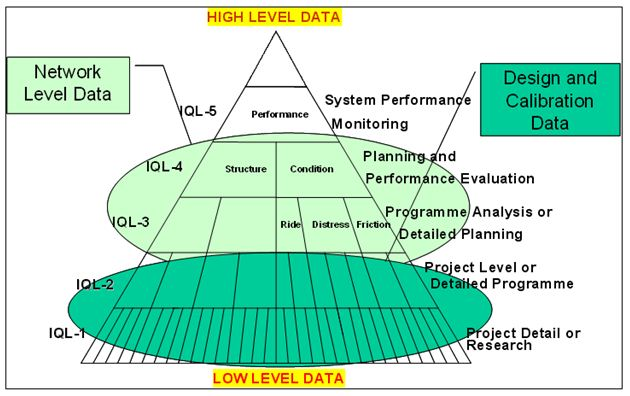
\includegraphics[scale=0.7]{iql}
\caption{Information Quality Level Conception}
\label{fig:Information Quality Level Conception}
\end{figure}

\clearpage
From the previous definition of IQL is possible to identify three observation.

\begin{itemize}

\item The higher the decision-level, the higher the IQL. Information at IQL-4 or IQL-5 is appropriate for performance indicators and road statistics, because of they are, easily understand without much technical background.
At the project-level, however, the appropriate IQL depends much on the standard of the project and the resources of the agency. For example, IQL-3 is usually sufficient for a rural road or a small local agency. For
most agencies and main roads, IQL-2 is typical, but for expressways, also IQL-1 may be used in some instances.
The criteria to select the appropriate IQL depends if the decision is altered by having more detailed information, and so with a different IQL level.

\item Primary data collection at a low-level (detailed) IQL typically costs more and involves more sophisticated instrument than the collection of higher IQL data. So, the IQL for primary data collection that is appropriate to a
given agency and situation depends on the financial and physical resources, skills, cost, speed or productivity, the degree of automation, complexity, all to obtain a  sustainable method, such as the regular operation of a road management system.

\item A higher level IQL often represents an aggregation or transformation of the lower level IQLs. When there is a specific rule or formula for conversion, from IQL-2 into IQL-3, then the information is reproducible and reliable. Thus, when the appropriate IQL is chosen, the
data can be re-used through a transformation to the higher IQLs and this avoids the need for repeating surveys and saves cost.


\end{itemize}
\clearpage
According to Bennett and Paterson\cite{bennett2000guide} was defined the following table of the amount of detail of each IQL level.

\begin{table}[ht]\label{tb:iql_detail}
\centering
    \begin{tabular}{ | l | p{15cm} |}

    \hline
    \textbf{IQL} & \hspace{5cm}
   \textbf{ Amount of Detail} \\ \hline


    \textbf{1} & \begin{footnotesize}
    The Most comprehensive level of detail, such as that which would be used as a
reference benchmark for other measurement methods or in fundamental
research. Would also be used in detailed field investigations for an in-depth
diagnosis of problems, and for high-class project design. Normally used at
project-level in special cases and unlikely to be used for network monitoring.
Requires high-level skill and institutional resources to support and utilize
collection methods.
    \end{footnotesize}\\
	\textbf{2} & \begin{footnotesize}
	A level of detail sufficient for comprehensive programming models and for
standard design methods. For planning, would be used only in sample coverage.
Sufficient to distinguish the performance and economic returns of different
technical options with practical differences in dimensions or materials. Standard
acquisition methods for project-level data collection. Would usually require
automated acquisition methods for network surveys and use for network-level
programming. Requires reliable institutional support and resources.
	\end{footnotesize} \\
	\textbf{3} &\begin{footnotesize}
	 Sufficient detail for planning models and standard programming models for full
network coverage. For project design, would suit elementary methods such as
catalogue-type with meagre data needs and low-volume road/bridge design
methods. Can be collected in network surveys by semi-automated methods or
combined automated and manual methods.
	\end{footnotesize}\\
	\textbf{4} & \begin{footnotesize}
	The basic summary statistics of inventory, performance, and utilization that are
of interest to providers and users. Suitable for the simplest planning and
programming models, but for projects is suitable only for standardised designs of
very low-volume roads. The simplest, most basic collection methods, either
entirely manual or entirely semi-automated, provide direct but approximate
measures and suit small or resource-poor agencies. Alternatively, the statistics
may be computed from more detailed data.
	\end{footnotesize} \\


\hline
    \end{tabular}
 \caption{Classification of Information by Quality and Detail}
\end{table}
\clearpage

\subsection{Quarter Car Model}\label{ssc:Quarter Car Model}
For the calculation of the IRI index, it is necessary to define a standard reference vehicle\cite{little_book}. This vehicle, for reasons of simplifying the index calculation process, was identified in the quarter-car model shown in Fig. \ref{fig:Quarter Car Model}. This model is two-dimensional because the only
movement in the $Z$ direction is taken into consideration. This model schematizes the vehicle with a sprung mass and a unsprung mass, connected by a shock absorber and a suspension, identified by a spring with own elastic constant and connected to the road pavement through the tire, also simplified with a spring of an elastic constant\cite{little_book}.

\begin{figure}[H]
\centering
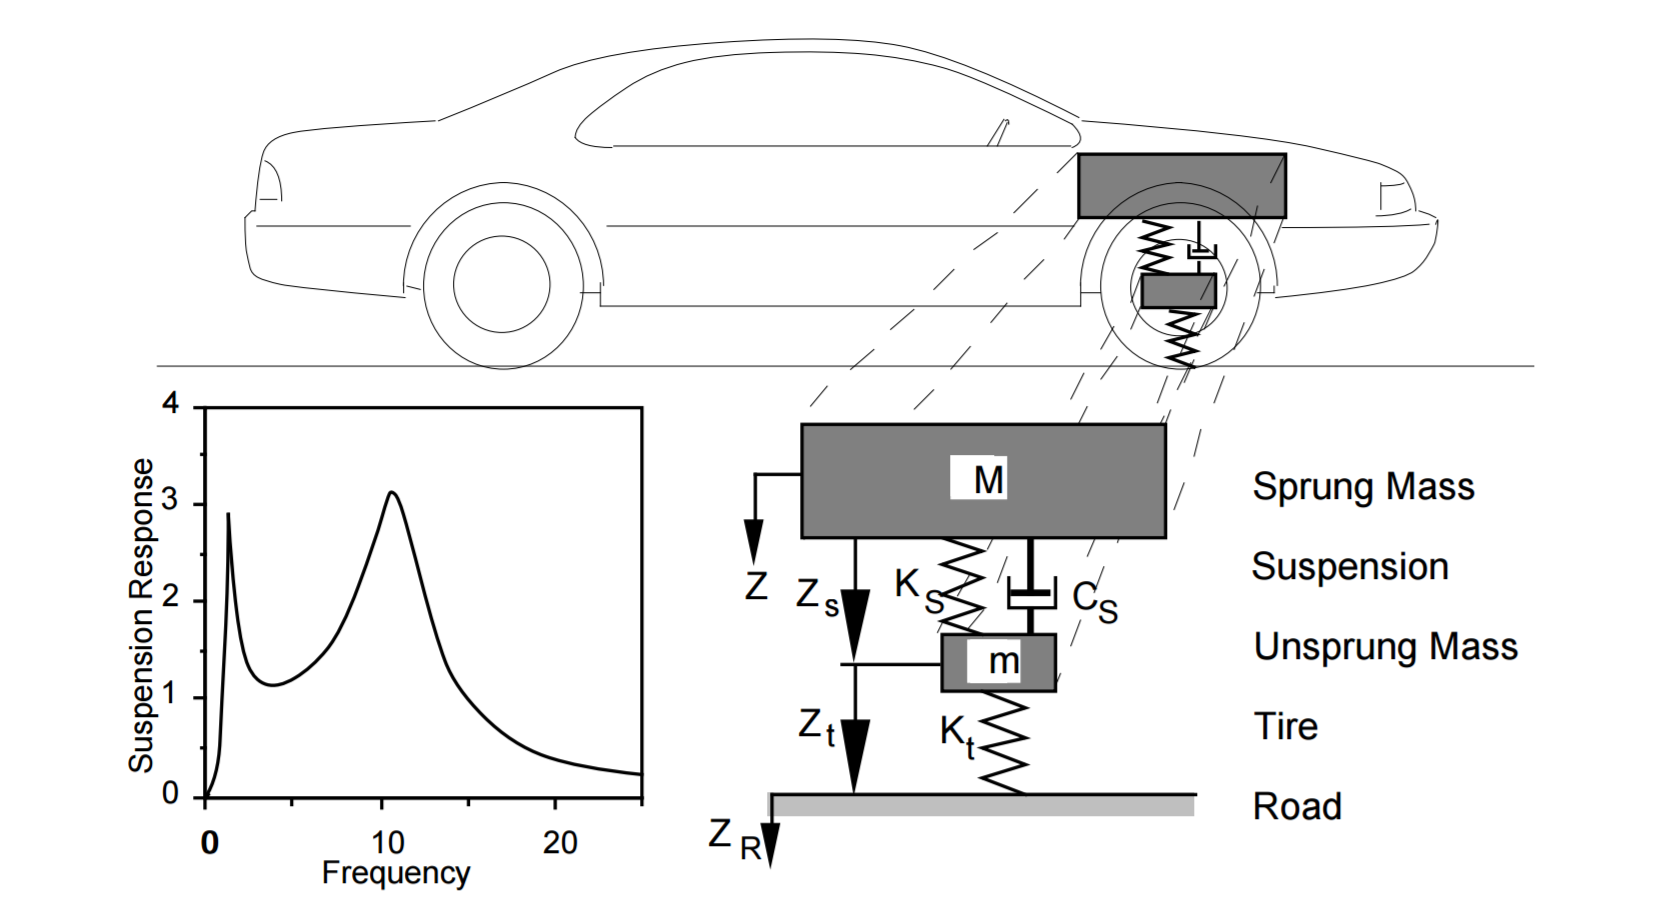
\includegraphics[scale=1]{quarter_car_model}
\caption{Quarter Car Model and Frequency Response}

\label{fig:Quarter Car Model}
\end{figure}

The roughness is seen as deviations in elevation\cite{gillespie1992everything} (displacement inputs), slope (velocity inputs), or change of slope (acceleration inputs), so the quarter car responds in a defined manner. The response can be mathematically described with a relatively simple set
of dynamic equations known as a quarter-car simulation.


\begin{center}

\[
    \left\{
                \begin{array}{ll}
                  \ddot{Z_{s}} m_{s} + C_{s} ( \dot{Z_{s}} - \dot{Z_{u}} ) + K_{s} (Z_{s} - Z_{u}) = 0\\
                   \ddot{Z_{u}} m_{u} + C_{s} ( \dot{Z_{u}} - \dot{Z_{s}}) + K_{s} (Z_{u} - Z_{s}) + K_{t} ( Z_{u} - Z_{p} ) = 0
                \end{array}
              \right.
\]




\end{center}

where the symbols represents:


$ Z_{s} =  $ The quote of sprung mass relative to the static equilibrium position,	\\
$ Z_{u} =  $ The quote of unsprung mass relative to the static equilibrium position,\\
$ Z_{p} = $ Road pavement height at fixed point,\\
$ m_{s} = $ Sprung mass,	\\
$ m_{u} = $ Unsprung mass, \\
$ k_{s} = $ Elastic subspension constant, \\
$ k_{u} = $ Elastic tire constant, \\
$C_{s} = $ Damper damping constant.\\

the system of two second order differential equations can be simplified by normalizing the parameters $mu$, $kt$, $ks$, $cs$ from the suspended mass $m_{s}$, according to the positions\cite{gillespie1992everything}:

        \begin{center}
       		$\mu = \dfrac{m_{u}}{m_{s}}; $ \quad
        	$k_{1} = \dfrac{k_{t}}{m_{s}} ; $ \quad
        	$k_{2} = \dfrac{k_{s}}{m_{s}} ; $ \quad
       		$c = \dfrac{C_{s}}{m_{s}}$
		\end{center}
leaving the equations in this form:

\begin{center}

\[
    \left\{
                \begin{array}{ll}
                  \ddot{Z_{s}} + C_{s} ( \dot{Z_{s}} - \dot{Z_{u}} ) + K_{1} (Z_{s} - Z_{u}) = 0\\
                  \ddot{Z_{u}} \mu + C_{s} ( \dot{Z_{u}} - \dot{Z_{s}}) + K_{2} (Z_{u} - Z_{s}) + K_{1}Z_{u}  = K_{1}Z_{p}
                \end{array}
              \right.
\]




\end{center}
thus, the system becomes a system of four differential equations of the first order that in matrix form can be expressed as:
\begin{center}
\[
\begin{bmatrix}
    \dot{Z_{s}}\\
    \ddot{Z_{s}} \\
    \dot{Z_{u}}\\
    \ddot{Z_{u}} \\
\end{bmatrix}
=
\begin{bmatrix}
    0 & 1 & 0 & 0 \\
    -k_{2} & -c & k_{2} & c \\
    0 & 0 & 0 & 1 \\
    \dfrac{k_{2}}{\mu} & \dfrac{c}{\mu} & -\dfrac{k_{1} + k_{2}}{\mu} & -\dfrac{c}{\mu} 
\end{bmatrix}
*
\begin{bmatrix}
    Z_{s}\\
    \dot{Z_{s}} \\
    Z_{u}\\
    \dot{Z_{u}} \\
\end{bmatrix}
+Z_{p}*
\begin{bmatrix}
    0\\
    0\\
    0\\
    \dfrac{k_{1}}{\mu} \\
\end{bmatrix}
\]
\end{center}

Where the resultant vector represents the vector of the state variables, i.e. the variables that are needed to fully define the state of the system. 
For the standard vehicle used in the IRI definition, the average values of American vehicles were obtained, this values obtained are called \textbf{\textit{"Golden Car"}}\cite{little_book}.
It presents the following coefficient values for the quarter of a vehicle:


\begin{table}[ht]\label{table:Golden Car Parameter}
\centering
    \begin{tabular}{ | l | l |}

    \hline
    Parameter  & Value \\ \hline


    $c$ & $6.0 \thinspace s^{-1}$\\ \hline
    $K_{1}$ & $653 \thinspace s^{-2}$\\ \hline
    $K_{2}$ & $63.3 \thinspace s^{-2}$\\ \hline
    $\mu$ & $0.15$\\ \hline

\hline
    \end{tabular}
 \caption{Golden Car Parameter}
\end{table}


About the frequency response of the model, at very low frequencies (corresponding to long wavelengths in the road) the suspension response is zero because the wheel and the vehicle body move up and down together. The response is maintained up through frequencies near $10$ $Hz$ where axle resonance occurs. Above the axle resonant frequency, the response again drops to zero as the road bumps simply deflect the tire without producing significant suspension stroke.
The frequency response of the quarter car extends from approximately $0.5$ to $20$ $Hz$.

\section{Calculation of IRI}\label{sc:Calculation of IRI}
Note the values, instant for instant, of the displacement velocities $Z_{s}$  and $Z_{u}$ obtained by integrating from the system of equations describing the motion of the Quarter car model, the calculation of the IRI is performed by the formula:
\begin{center}
{\LARGE $IRI = \frac{1}{L} \int_{0}^{\frac{L}{V}} | \dot{Z_{s}} - \dot{Z_{u}} | dt$}
\end{center}
where $L$ is the profile length and $V$ is the standard speed of $\num{80} \si{\km\per\hour}$. Generally IRI is measured in $\si{\milli\meter\per\km}$ or in  mile$^{-1}$. This index, as defined, is comparable to two profiles, meaning that if a $500$ $\si{\meter}$ profile has an IRI index of $100$ $\si{\milli\meter\per\km}$ and the next $500$ \thinspace \si{\meter} profile has an IRI index of $200$\thinspace\si{\milli\meter\per\km}, The entire $1000$\si{\meter} profile will have an IRI of $150$ $\si{\milli\meter\per\km}$, and this is one of the most important features\cite{little_book} of that index. 

The measurement and calculation procedure of IRI are also based on the following principles:
\begin{itemize}

\item A single longitudinal profile with sample interval not longer than $300$ $\si{\milli\meter}$ is measured.
\item The measured profile is smoothed with a $250$\si{\milli\meter} base length moving average filter known as IRI filter.
\item The slope between consecutive elevation points is considered to be constant.

\end{itemize}
The IRI index is calculated by filtering the measured profile with the quarter car filter, at a simulation speed of $\num{80} \si{\km\per\hour}$, so that it provides a summary value of the slope, as it is recorded by the vehicle. The algorithm used for the IRI value calculation uses a theoretical filter describing the quarter car theoretical response to pavement surface irregularities.

As mentioned briefly earlier, the IRI index has been defined to classify road pavements in terms of driving comfort in the vehicle and damage to the pavement. Indeed, the correlation between IRI and comfort or damage is remarkable\cite{gillespie1992everything}.




\end{document}